\documentclass[10pt]{beamer}
\usepackage[utf8]{inputenc}

\usetheme{metropolis}

\usepackage{acronym} % \ac[p], \acl[p], \acs[p], \acf[p]
\usepackage{appendixnumberbeamer}
\usepackage[scale=2]{ccicons}
\usepackage[absolute, overlay]{textpos}

\usepackage{caption}
\usepackage{url}

\setbeamertemplate{caption}[default]
\setbeamertemplate{bibliography item}[text]

% Acronyms
% --------
\acrodef{CRDT}[CRDT]{Conflict-free Replicated Data Type}
\acrodefplural{CRDT}[CRDTs]{Conflict-free Replicated Data Types}

% Metadata
% --------
\author{
  Matthieu Nicolas
}
\title{Efficient renaming in \acp{CRDT}}
\institute{}

\begin{document}

\begin{frame}[t,plain]
  \maketitle
\end{frame}

\begin{frame}{LogootSplit\cite{AndreCollaborateCom2013}}
  \begin{itemize}
    \item State of the art of \emph{Sequence \acfp{CRDT}}\cite{shapiro_2011_crdt}
    \item Allows nodes from a distributed system to replicate and edit sequences without any coordination
    \bigskip
    \item Relies on \emph{identifiers} to ensure convergence
  \end{itemize}
\end{frame}

\begin{frame}{Identifier-based approach}
  \begin{block}{Main idea}
    \begin{itemize}
      \item Generate and attach an identifier to each inserted element
    \end{itemize}
  \end{block}

  \bigskip

  \begin{block}{Allow to achieve commutative updates}
    \begin{itemize}
      \item By identifying uniquely elements
      \item By ordering them relatively to each other
    \end{itemize}
  \end{block}
\end{frame}

\begin{frame}{Identifier constraints}

  \begin{itemize}
    \item To fulfill their role, identifiers have to comply to several constraints:
  \end{itemize}

  \begin{block}{Globally unique}
    \begin{itemize}
      \item Identifiers should never be generated twice, neither by different users nor by the same one at different times
    \end{itemize}
  \end{block}
  \begin{block}{Totally ordered}
    \begin{itemize}
      \item We should always be able to compare and order two elements using their identifiers
    \end{itemize}
  \end{block}
  \begin{block}{Dense set}
    \begin{itemize}
      \item We should always be able to add a new element, and thus a new identifier, between two others
    \end{itemize}
  \end{block}
\end{frame}

\begin{frame}{LogootSplit identifiers}
  \begin{itemize}
    \item To comply with these constraints, LogootSplit proposes identifiers composed of quadruplets of integers of the following form:
  \end{itemize}
  \begin{center}
    $<priority, siteId, seq, offset>$
  \end{center}
  \begin{itemize}
    \item \emph{priority} allows to determine the position of this identifier compared to others
    \item \emph{siteId} refers to the node's identifier, assumed to be unique
    \item \emph{seq} refers to the node's logical clock, which increases monotonically with local operations
    \item \emph{offset} refers to the element position in its original block
  \end{itemize}
\end{frame}

\begin{frame}{State of a LogootSplit sequence}

  \begin{itemize}
    \item The state of such sequence corresponds to the elements contained in the sequence and their respective identifier
    \item For simplicity purpose, we will use letters instead of quadruplets of integer to represent identifiers
    \item We represent the state of a given sequence as the following:
  \end{itemize}

  \begin{figure}
    
\includegraphics[scale=0.15]{img/helo-as-letters.png}
    \caption{The state of a sequence which contains the elements "helo" and their corresponding identifiers}
  \end{figure}

\end{frame}

\begin{frame}{Blocks}

  \begin{itemize}
    \item To reduce the identifiers' footprint, LogootSplit aggregates elements with \emph{contiguous} identifiers into blocks
    \item Two identifiers are \emph{contiguous} iff
    \begin{itemize}
      \item They have the same size
      \item All their components but their last $offsets$ are equal
      \item Given their respective last offsets $o$ and $o'$, $o$ is the successor of $o'$ or conversely
    \end{itemize}
    \item It allows to reduce the metadata stored to only the identifier of the first element of the block and the last $offset$ of the last element
    \item We represent blocks as the following:
  \end{itemize}

  \begin{figure}
    
\includegraphics[scale=0.15]{img/helo-as-block.png}
    \caption{The state of a sequence which contains the block "helo"}
  \end{figure}

\end{frame}

\begin{frame}{Operations}
  \begin{itemize}
    \item Two local operations are defined on the data structure
    \begin{itemize}
      \item $insert$ allows a node to add elements at a given position. It generates and attaches identifiers to inserted elements.
      \item $delete$ allows a node to remove an interval of elements and their identifiers.
    \end{itemize}
  \end{itemize}
  \begin{figure}
    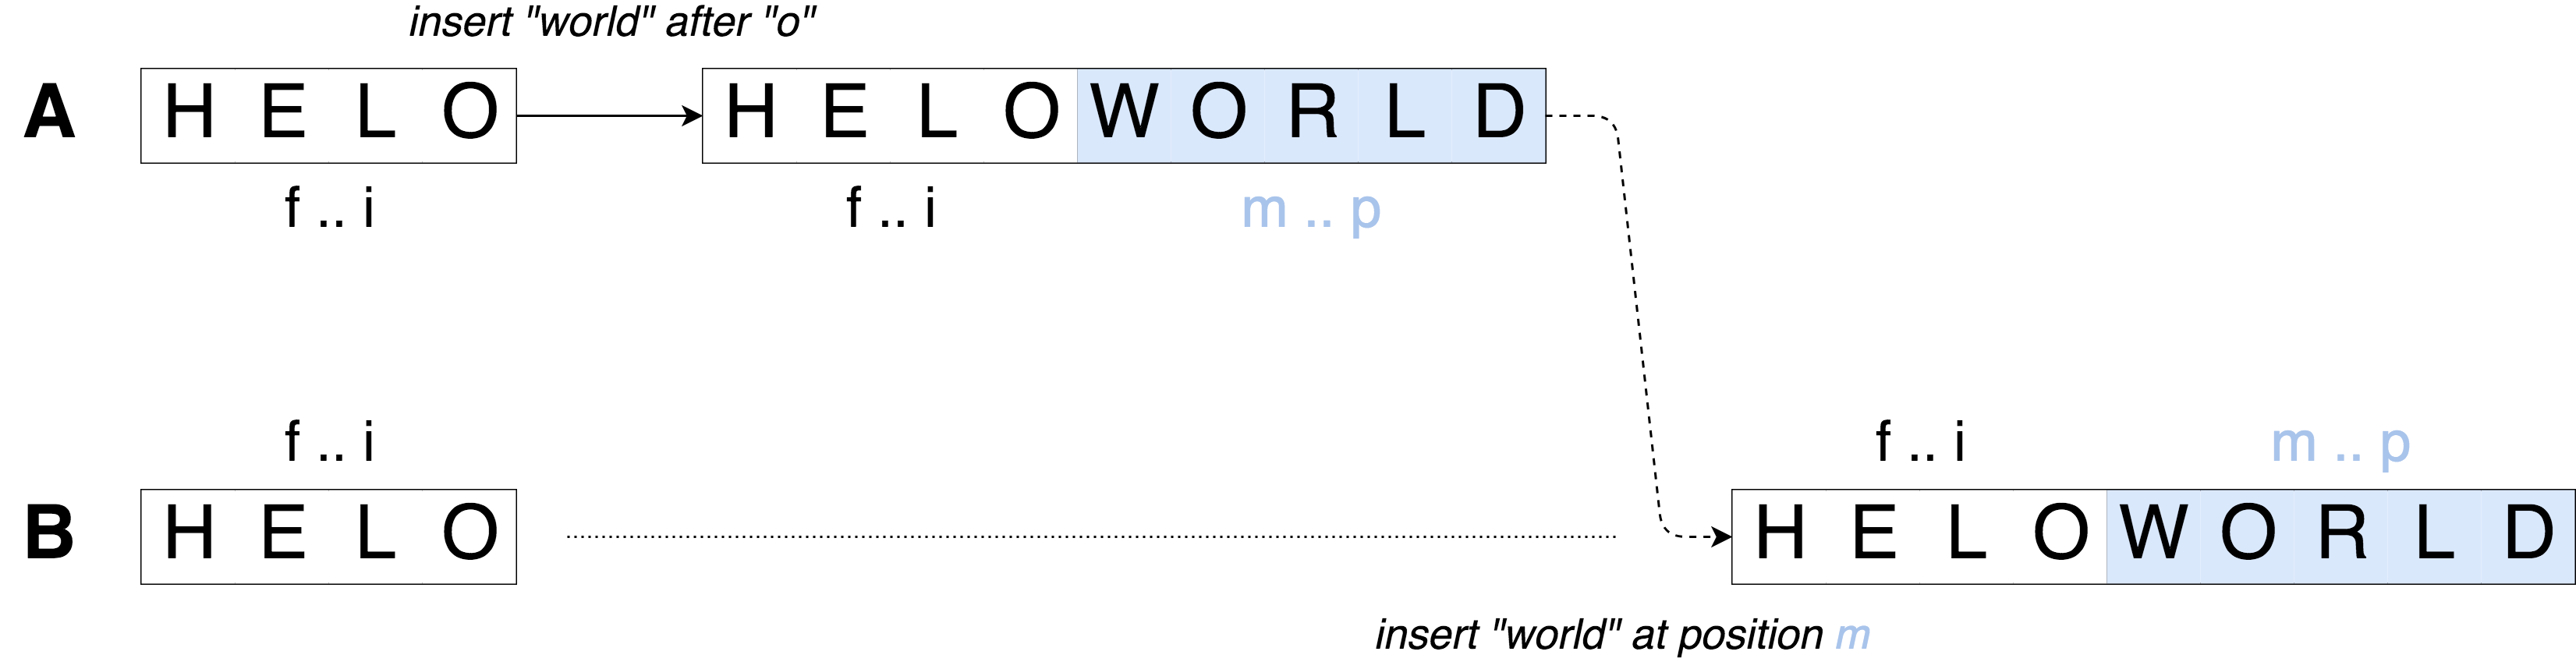
\includegraphics[scale=0.09]{img/insert.png}
    \caption{Example of $insert$ operation}
  \end{figure}
  \begin{itemize}
    \item Each local operation is then propagated to other nodes, using identifiers instead of simple integers as positions to ensure convergence
  \end{itemize}
\end{frame}

\begin{frame}{Growing identifiers}
  \begin{itemize}
    \item However, a node may try to insert a new element between two others with contiguous identifiers
    \begin{itemize}
      \item For example, between the identifiers \emph{g} and \emph{h}
    \end{itemize}
    \item There is no mean to generate a new identifier \emph{id} of same size such as $g < id < h$
    \item To generate a fitting identifier, LogootSplit concatenates the predecessor's identifier to a newly generated quadruplet of integers
    \begin{itemize}
      \item For example, $g$ is concatenated to $m$ to generate a valid identifier
    \end{itemize}
  \end{itemize}
  \begin{figure}
    
\includegraphics[scale=0.15]{img/insert-between.png}
    \caption{Insertion leading to the generation of longer identifiers}
  \end{figure}
\end{frame}

\begin{frame}{Declining performances}
  \begin{itemize}
    \item Operations performed may lead to an inefficient internal representation
    \item With blocks containing few elements...
    \item ... and using long identifiers
  \end{itemize}
  \begin{figure}
    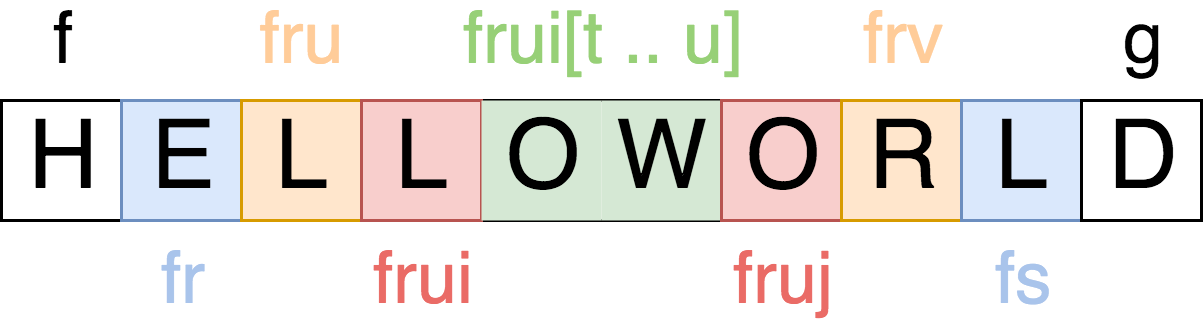
\includegraphics[scale=0.15]{img/worst-case.png}
    \caption{Example of inefficient internal representation}
  \end{figure}
  \begin{itemize}
    \item The more blocks we have:
    \begin{itemize}
      \item The more metadata we store
      \item The longer it takes to browse the sequence to $insert$ or $delete$ an element
    \end{itemize}
  \end{itemize}
\end{frame}

\begin{frame}{Renaming}
  \begin{itemize}
    \item To address this issue, propose to introduce a $rename$ operation
    \item This operation reassigns an identifier composed of one quadruplet of integers to the first element, based on his previous identifier
    \item It then generates contiguous identifiers for all following elements
    \item This allows to aggregate all elements in one block
    \begin{itemize}
      \item Reducing the metadata footprint to the identifier of the first element and the $offset$ of the last one
    \end{itemize}
  \end{itemize}
  \begin{figure}
    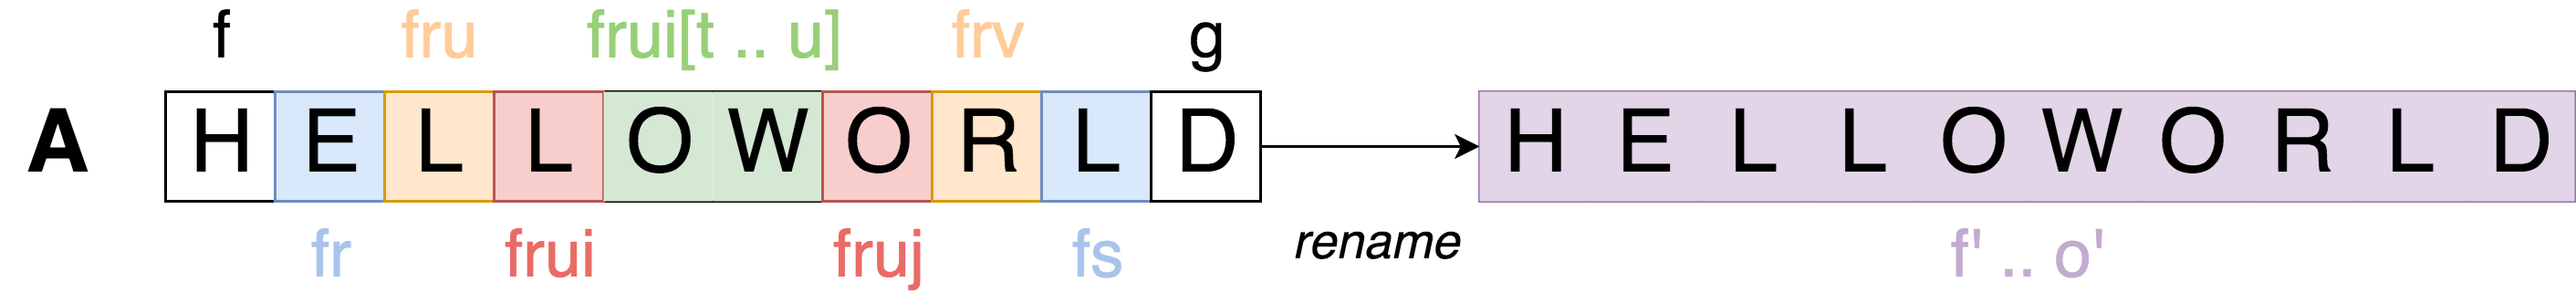
\includegraphics[scale=0.11]{img/renaming.png}
    \caption{Example of renaming}
  \end{figure}
\end{frame}

\begin{frame}{Handling concurrent operations}
  \begin{itemize}
    \item However, additional metadata is temporary required to handle concurrent operations
    \item This metadata is used to compute rewriting rules for identifiers inserted or deleted by other nodes concurrently
    \item It can be garbage collected once every node has observed the $rename$ operation
  \end{itemize}
\end{frame}

% \begin{frame}{Example}
%   \begin{itemize}
%     \item By propagating the inserted elements and their identifiers, nodes are able to converge
%   \end{itemize}
%   \begin{figure}
%     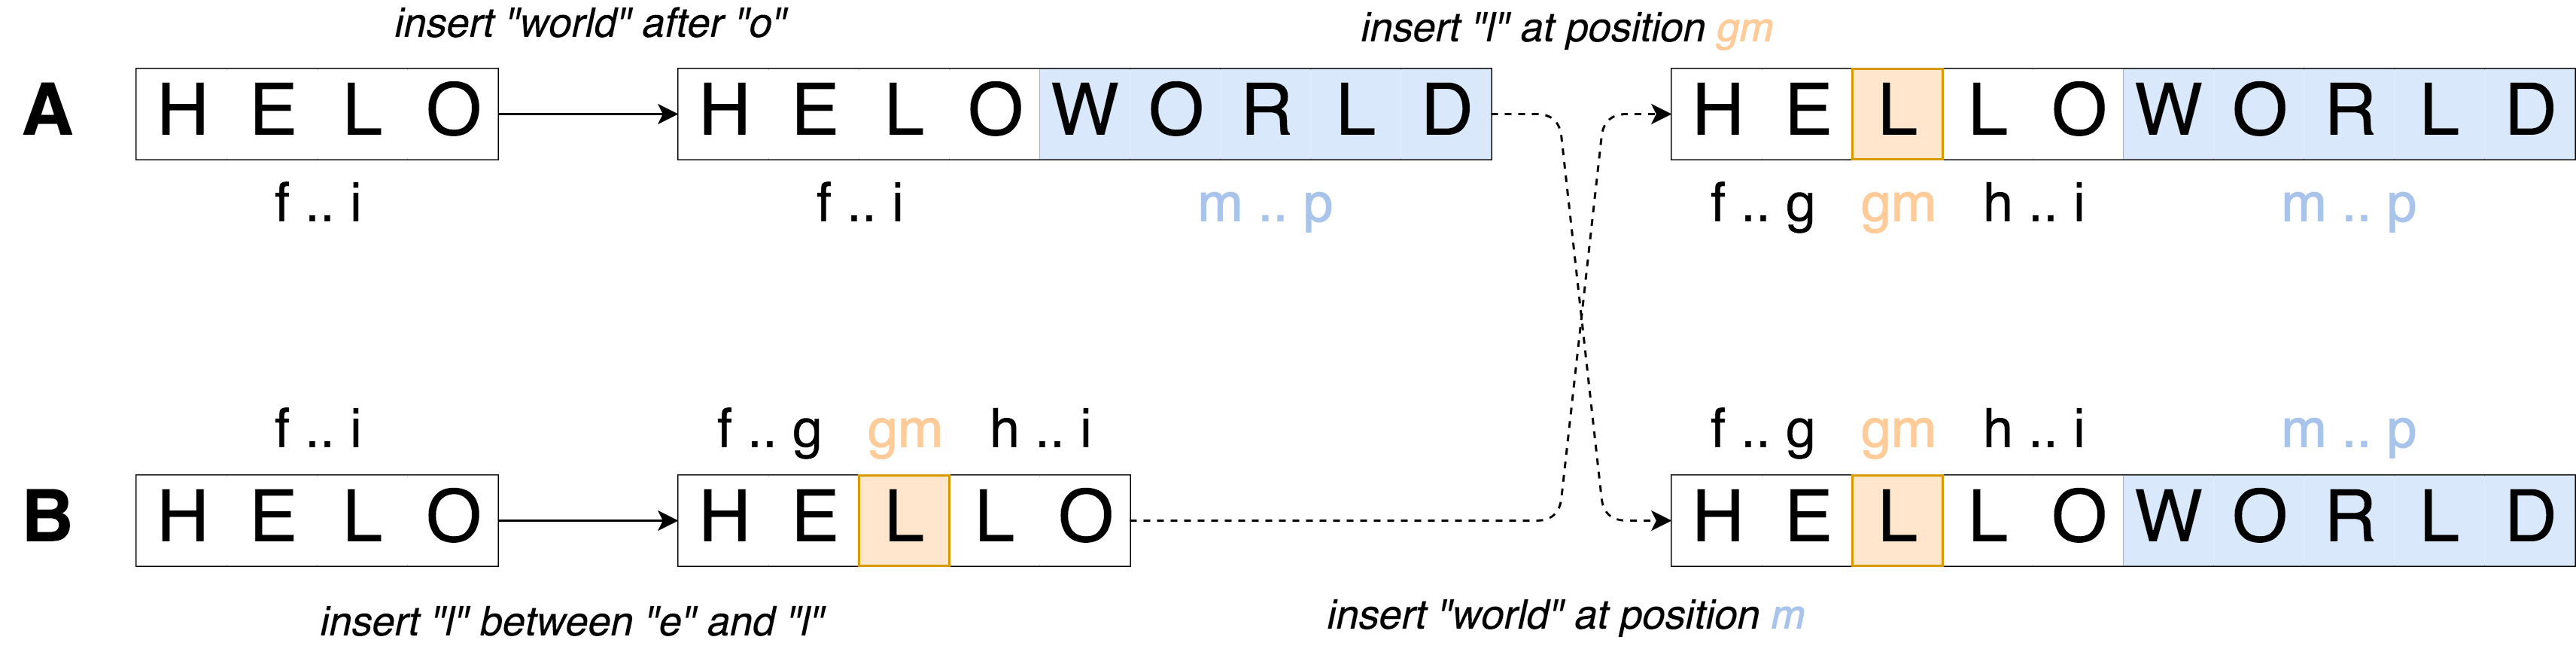
\includegraphics[scale=0.09]{img/concurrent-inserts.png}
%     \caption{Concurrent inserts are commutative by design}
%   \end{figure}
% \end{frame}

\begin{frame}[standout]
  Thanks for your attention!
  \vspace{3em}
  \begin{center}
    \ccby
  \end{center}
\end{frame}

\begin{frame}[allowframebreaks]
  \frametitle{References}
  \bibliographystyle{abbrv}
  \bibliography{biblio}
\end{frame}

\end{document}

% \begin{frame}{Exemples}
%   \only<1> {
%     \begin{figure}
%       \includegraphics[scale=0.25]{img/search-results-google.png}
%       \caption{Résultats d'une recherche Google}
%     \end{figure}
%   }
%   \only<2>{
%     \begin{figure}
%       \includegraphics[scale=0.20]{img/timeline-twitter.png}
%       \caption{Timeline Twitter}
%     \end{figure}
%   }
% \end{frame}
